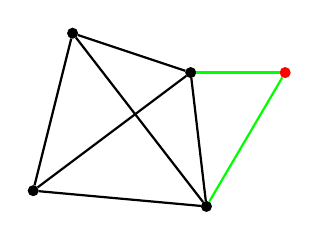
\begin{tikzpicture}[
  dot/.style = {
    shape = circle,
    fill = black,
    minimum size = 4pt,
    inner sep = 0pt,
    outer sep = 0pt,
  },
  every path/.style = {
    thick
  }
]
  \node[dot] (v1) at (-1, 0) {};
  \node[dot] (v2) at (-0.5, 2) {};
  \node[dot] (v3) at (1, 1.5) {};
  \node[dot] (v4) at (1.2, -0.2) {};

  \draw (v1) -- (v2) -- (v3) -- (v4) -- (v1) -- (v3);
  \draw (v2) -- (v4);

  \node[dot, fill = red] (v5) at (2.2, 1.5) {};
  \draw[very thick, green] (v5) edge (v3) edge (v4);
\end{tikzpicture}